
\begin{section}{Geometry Generation}
\label{sec:workflow-geometries}


\begin{subsection}{Guiding Principles}


For any given monomer(s) of interest, the first step in the force field
development process is to choose a series of optimal dimer
configurations. This `optimal' set is highly dependent on the type of force field that
is being fit, and indeed the recommendations offered below are specific to the
\sapt-based force fields described in \cref{ch:isaff,ch:mastiff}.

\begin{figure}
\centering
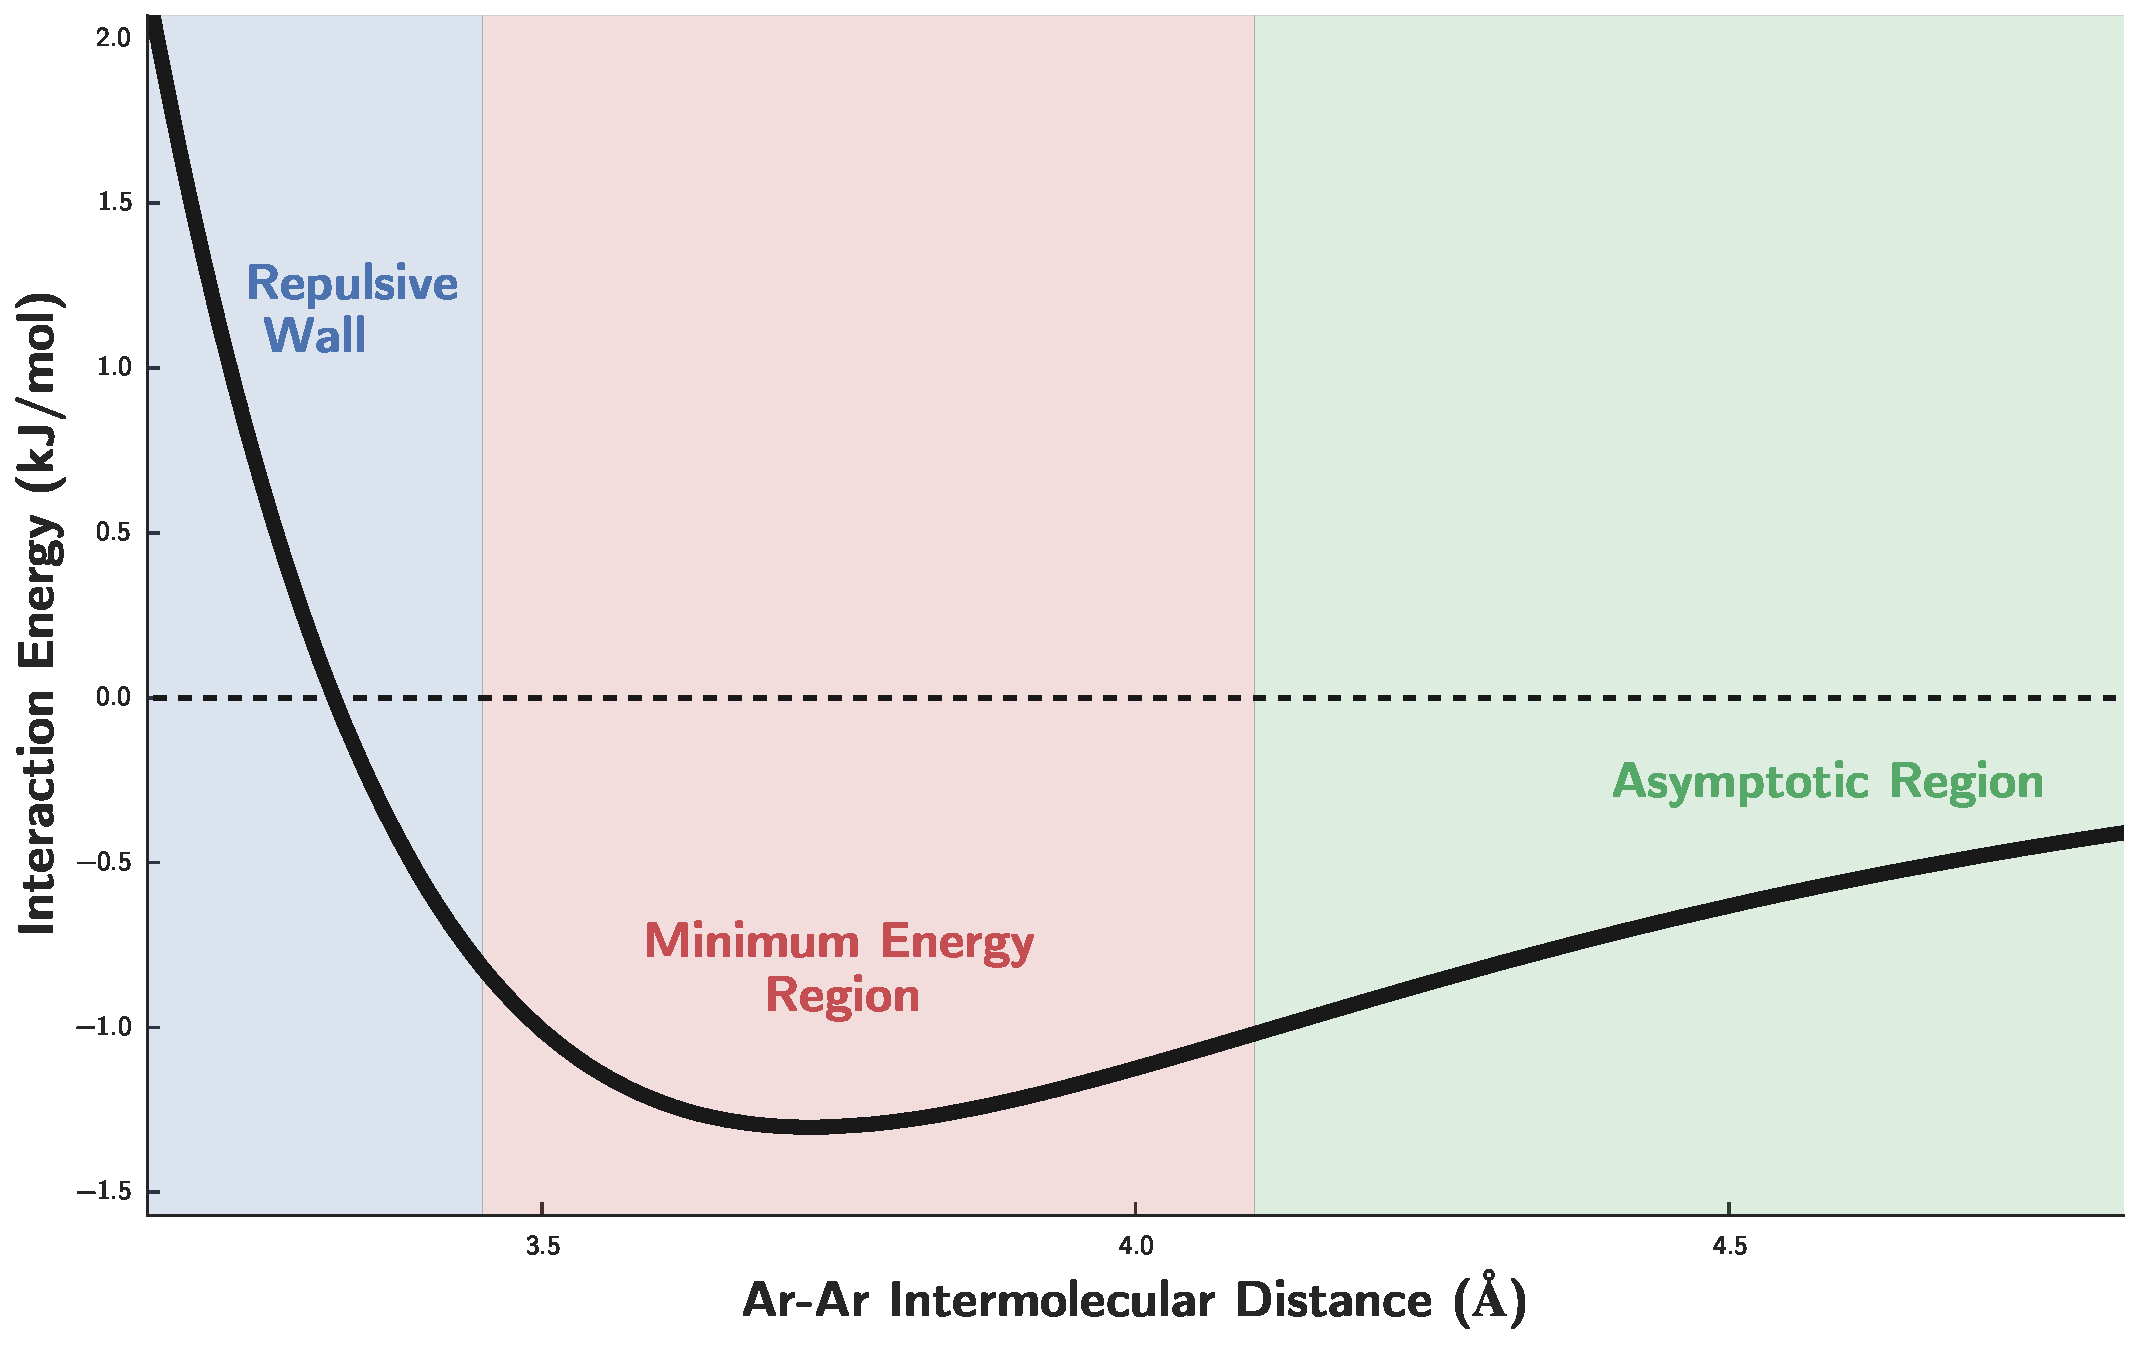
\includegraphics[width=1.0\textwidth]{workflow/generalized_pes.pdf}
\caption[Generalized form of a \pes showing the repulsive wall, minimum
energy, and asymptotic regions.]
        {Generalized form of a \pes showing the repulsive wall, minimum
energy, and asymptotic regions of the argon dimer. Cutoffs between the
different regions should be taken qualitatively.}
\label{fig:workflow-pes}
\end{figure}

In general, and as shown in \cref{fig:workflow-pes}, a given \pes will have
(qualitatively) three different regions: a repulsive wall, a minimum energy
region, and an asymptotic region. (Energies in the asymptotic region are
usually attractive, but are sometimes repulsive due to unfavorable
electrostatic interactions). 
Based on the principles of statistical mechanics and the Boltzmann
distribution, we know that (for a system
at constant temperature $T$) the probability $P_i$ of observing a system in state
$i$ is exponentially-dependent on the energy of that state:\cite{Frenkel2002}
%
\begin{align}
P_i \propto exp(-E_i/k_B T)
\label{eq:workflow-boltzmann}
\end{align}
%
where $k_B$ is the Boltzmann constant.

Due to the exponential relationship between the energetic stability of a given
state and the probability of experimentally observing said state, \emph{routine molecular simulation will most frequently
sample dimer configurations near the minimum energy and asymptotic
regions of the potential}.\footnotemark{} Consequently,
these two portions of the \pes are the most important to accurately model with
a force field.
%
\footnotetext{
Although it's straightforward to see why the minimum energy region gets
sampled in molecular simulation, the importance of the asymptotic region 
may be hard to understand simply by looking at
\cref{eq:workflow-boltzmann} and the 2-body \pes shown in \cref{fig:workflow-pes}. 
We should recognize, however, that the two-body energy of an $N$-body system is
determined both by nearest neighbor interactions (whose configurations are
typically in the minimum energy region of the 2-body \pes) and by the more
distant, non-nearest neighbor interactions (whose configurations lie in the
asymptotic region). The number of non-nearest neighbor interactions outweigh
the closer-contact interactions, which in turn makes \emph{both} the minimum
energy and asymptotic regions of the potential important to correctly model.
}
%
Nevertheless, and as discussed in \cref{sec:workflow-monomer_parameters}, the
asymptotic region of the \pes primarily depends on well-known functionals forms whose
parameters are calculated from monomer properties, making 
the dimer-based fits described in \cref{ch:pointer} relatively insensitive to
inclusion of configurations in this %region.
region.\footnote{By contrast, other functional forms (e.g. Lennard-Jones) \emph{do}
have parameters that effect the asymptotic region, and for these force fields
it would be important to include this region in the parameterization process.}
%
By contrast, the force field parameters we directly fit to the dimer \pes are
primarily sensitive to the shape and location of
the repulsive wall and (to a lesser extent) the minimum energy
regions.
Consequently, and based on the combination of their observation probability in molecular
simulation as well as their importance in the improving the force field fitting process,
\emph{dimer configurations along the repulsive wall and (even more
importantly) in the minimum energy region are the
most important to parameterize in order to develop highly-accurate force fields}.\footnotemark{}

\footnotetext{Historical note: For force field functional forms which
poorly model the repulsive wall (e.g. Lennard-Jones force fields or the \saptff
described in \cref{ch:isaff}), 
the force field fit quality strongly depends on the
relative representation of repulsive and attractive dimer configurations,
and including either too few or too many repulsive configurations can be
problematic. Only with the advent of \isaffold and \mastiff is the
fit quality strictly improved by including repulsive configurations.}


In practice, a standard procedure for optimally sampling across the
\pes has been established for the \isaffold
and \mastiff force fields. Though use of different functional forms might
require a different relative sampling of the dimer \pes, the next sections completely outline the
theory and practical calculations that are involved in generating dimer
configurations for the development of \isaffold and \mastiff force fields.

\end{subsection}
\begin{subsection}{Theory}

Assuming rigid monomer geometries, a dimer configuration can be completely
determined (without loss of generalization) by fixing the center of the first monomer at the
origin and by placing the second monomer according to six variables. $r$, $\theta$, and $\phi$ determine the position
of the center of the second monomer, and the three-dimensional variable $\Omega$ determines the relative
orientation of this second monomer about its center. In practice, $\Omega$ is
most easily described by a quaternion, and the interested reader is referred
to \citen{Guibas1992} for details.

For both the \isaffold and \mastiff fits, dimer configurations are sampled
psuedo-randomly using Shoemake's algorithm,\cite{Shoemake1992} which ensures
even sampling of the dimer configurations. 
Additionally, and
in order to achieve a proper balance of sampling between the
repulsive wall and minimum energy regions, and in order to largely prevent
the asymptotic region from being sampled, the following dimer configurations
are excluded from sampling:
\begin{enumerate}
\item Configurations with any atom-atom contact distance 
$r_{ij} \le 0.8\times(r^{\text{vdw}}_i + r^{\text{vdw}}_j)$, where $r_{ij}$ is the
contact distance and $r^{\text{vdw}}$ is the tabulated van der Waals radius
for a given element
\item Configurations with all atom-atom contact distance 
$r_{ij} \ge 1.3\times(r^{\text{vdw}}_i + r^{\text{vdw}}_j)$.
\end{enumerate}
A working code for this sampling algorithm has been developed and is described
in the next Section.  Given the large number ($\approx 1000$) of points we
typically sample for each new force field, this simple sampling algorithm is
usually sufficient for obtaining high-quality force fields.  In the future,
however, it may be worthwhile to adopt more sophisticated and efficient
sampling algorithms, as this might allow us to substantially reduce the number
of required dimer configurations.\cite{Metz2016}


\end{subsection}
\begin{subsection}{Practicals}

Insofar as user input is concerned, generating dimer configurations is
reasonably straightforward.
After downloading the Workflow from GitHub, 
the user will have access to the following subdirectories:
\begin{lstlisting}[language=bash]
$ ls
documentation  input  scripts  templates
\end{lstlisting}
The three required input files for geometry generation -- \verb|input/dimer_info.dat|,
\verb|input/generate_grid_settings.inp|, and \verb|input/<mona>_<monb>.inp| --
are
listed  in
\cref{lst:workflow-generate_geometries,lst:workflow-dimer_info,lst:workflow-dimer_geom}
using the pyridine dimer as an example.
(Here and throughout, we use angle brackets to indicate required arguments.)
Each input file may need to be modified for the specific dimer under consideration, and
comments within these input files explain any necessary system-specific changes.

Once all required input files have been created/modified, the geometry generation process can
be carried out very simply from the main Workflow directory by
executing the command
%
\begin{lstlisting}
./scripts/make_geometries.sh
\end{lstlisting}

\end{subsection}


\end{section}
